\section{Methodology}
\label{sec:methodology}

\subsection{Data}

This study used two datasets: the main dataset from StreetSwipe \cite{streetswipe}, and an extended dataset of other areas in Amsterdam. An illustration of the areas covered by each dataset can be seen in Figure \ref{fig:map}.

{
\setlength{\intextsep}{0pt}
\begin{figure}[h!]
    \centering
    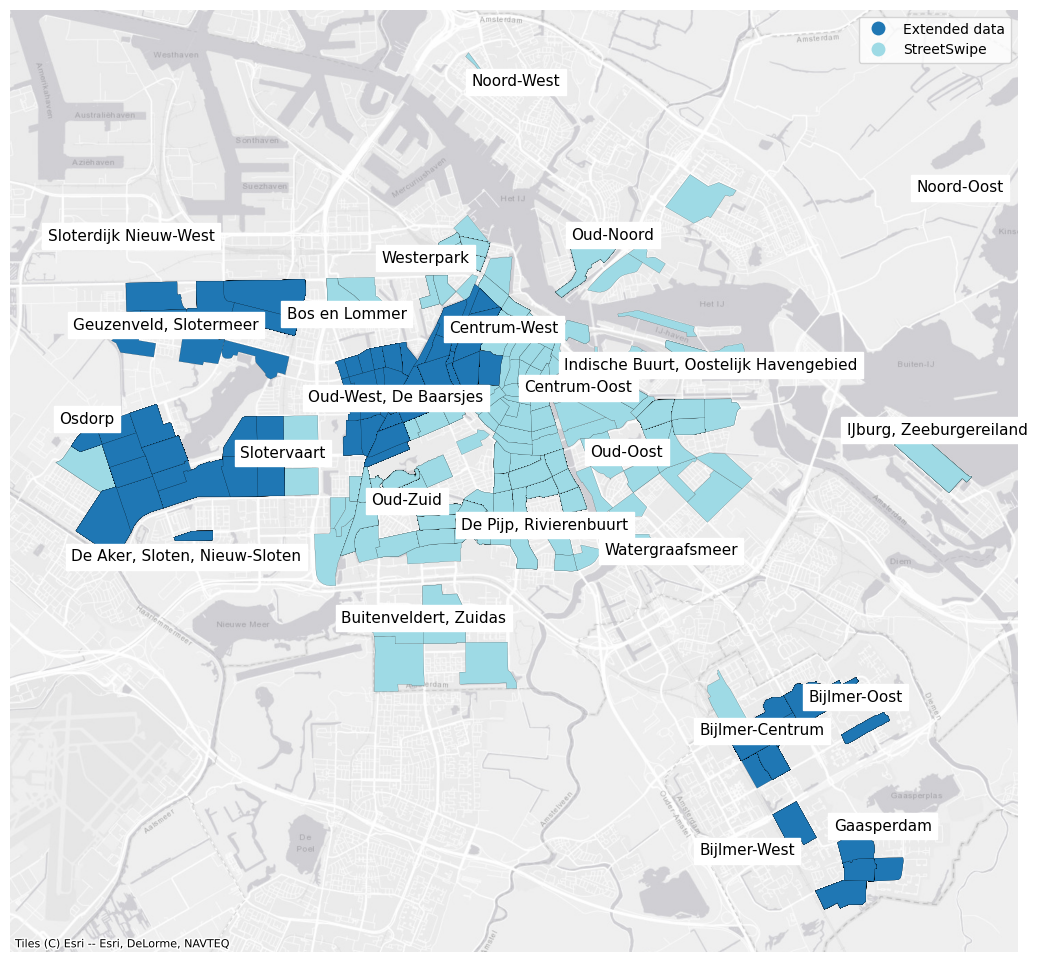
\includegraphics[width=0.5\textwidth]{media/methodology/map/map2.png}
    \caption{Areas of Amsterdam present in StreetSwipe and the extended dataset. StreetSwipe had images mainly from the city center (Centrum-Oost and -West), Oost, and Zuid. The extended dataset had images taken from Centrum-West (Jordaan), Oud-West, De Baarsjes, Nieuw-West, and Zuidoost.}
    \label{fig:map}
\end{figure}
}

\subsubsection{StreetSwipe}
StreetSwipe's images were originally from Google Street View, which were cropped to focus on facades (examples are in Figure \ref{fig:SS_example}. Using crowd-sourcing, the project lets people decide whether each facade appear gentrified, by voting "Yes" or "No" on the images. The official \textit{Gentrified} and \textit{Non-gentrified} label per facade are based on what the majority voted for. Thus, this dataset represents common visual perception of gentrification.  

\begin{figure}
    \begin{tabular}{cccc}
        \subfloat{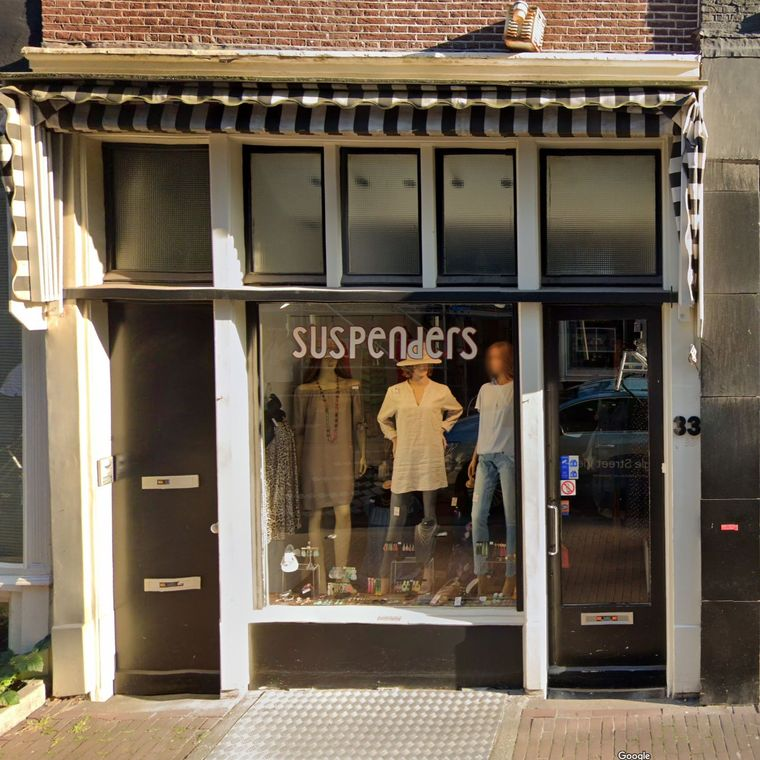
\includegraphics[width = 1.55in]{media/methodology/data_ex/SS/gen1.jpg}} &
        \subfloat{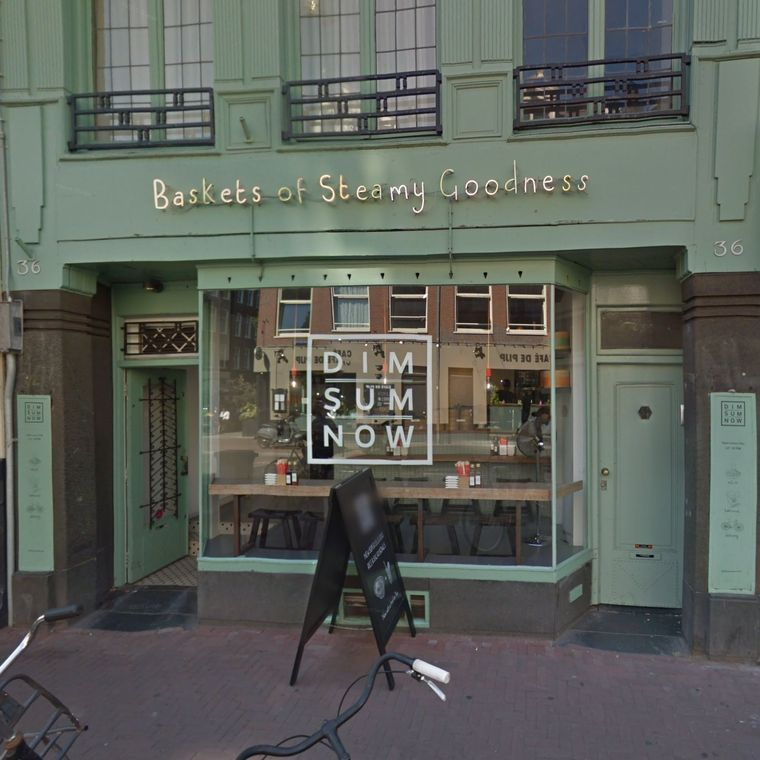
\includegraphics[width = 1.55in]{media/methodology/data_ex/SS/gen2.jpg}} \\
        \subfloat{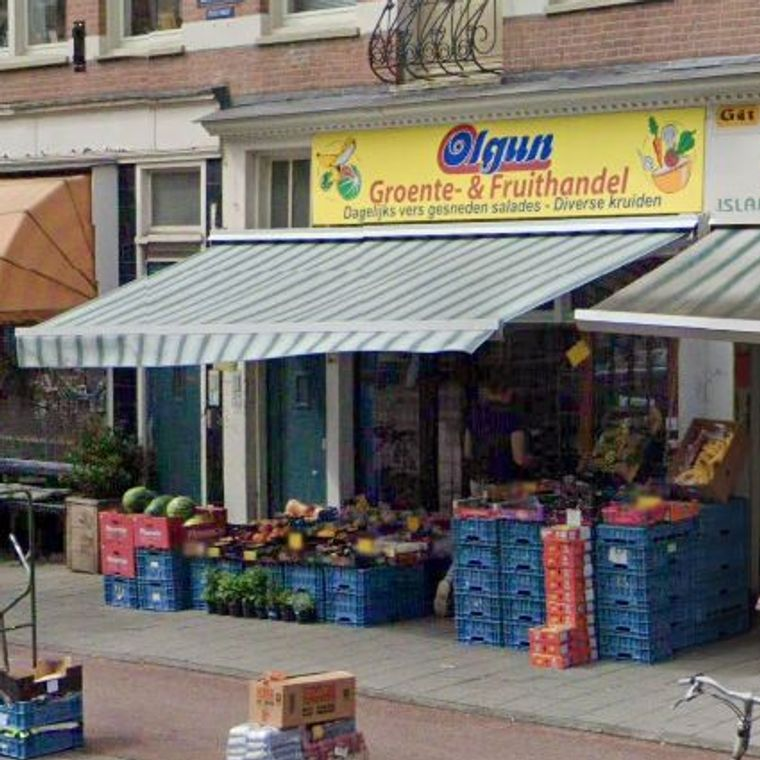
\includegraphics[width = 1.55in]{media/methodology/data_ex/SS/non1.jpg}} &
        \subfloat{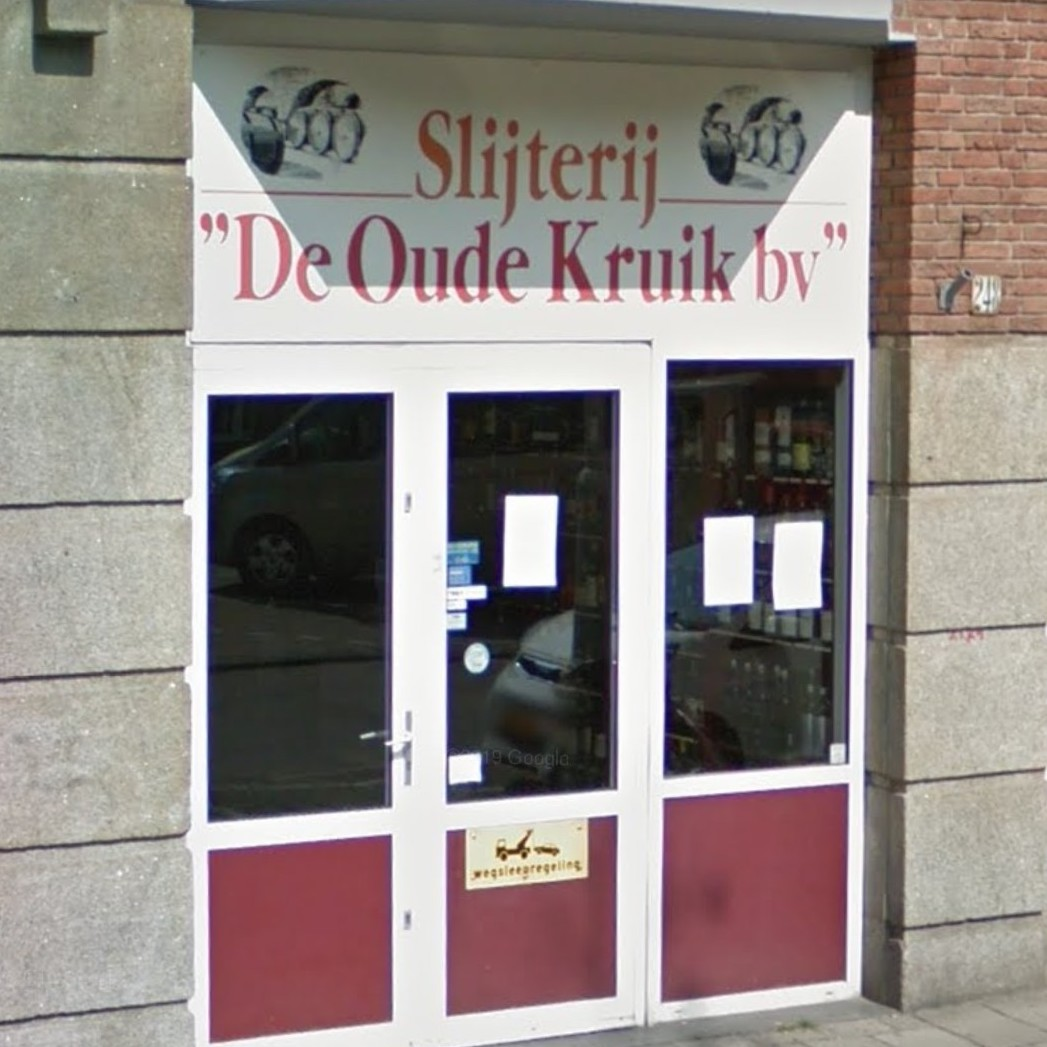
\includegraphics[width = 1.55in]{media/methodology/data_ex/SS/non3.jpg}} \\
    \end{tabular}
    % \vspace{\baselineskip}
    \caption{Examples of StreetSwipe images.}
    \label{fig:SS_example}
    \vspace{-5mm}
\end{figure}

Since there were two versions of StreetSwipe, the data retrieved existed in two sets: 1912 higher resolution images from the older version, and 529 lower resolution images from the new one. The dataset thus had 2441 images in total, each with its numbers of "Yes" and "No" votes, and metadata on the facade's coordinates and street name. The new version's images also had more detailed address, name, and type of business/services. There were also more votes in the new version than in the old one. The images from the old version were available directly, while the new ones were provided via URLs to a Google APIs bucket, and thus were scraped.

Feature engineering was done to create the gentrified/ non-gentrified labels, by taking the vote higher in volume. The images were then re-grouped per their corresponding labels. There was class imbalance in the data, with 71\% of the images being non-gentrified (1731 images; versus 710 gentrified images). The images had quite consistent aspect ratios of approximately 1:1; however, they varied in size, ranging from around 300x300 to 1700x1700, with one outlier of size 2500x1300, approximately.


\subsubsection{Extended data}

Data from areas not present in StreetSwipe was used to test the model's generalizability. Given literature on gentrification in Amsterdam, gentrified and non-gentrified neighborhoods were selected, and street view images from these areas were retrieved from a dataset made available by the Civic AI Lab.

Using Dutch resident register data, Hochstenbach and Van Gent \cite{hochstenbach_anatomy_2015} identified gentrification in Amsterdam's neighborhoods via residential mobility (characteristics of neighborhood's in-movers and out-movers), social mobility (change in current residents' socio-economic situation), and neighborhood's demographic changes (age, income) over the 2004-11 period. Following these indicators, downgrading neighborhoods (i.e. declined median income) were found to be in Zuidoost and Nieuw-West; and no trend of social mobility and displacement was found in these areas. Upgrading neighborhoods (i.e. increased median income) were largely in Oud-West, De Baarsjes and Centrum-West - particularly De Jordaan; and these areas underwent social mobility and displacement (see Appendix \ref{sec:apx:Hochstenbach} for visualizations of these findings). Thus, Zuidoost and Nieuw-West were selected as non-gentrified areas; and De Jordaan, Oud-West, and De Baarsjes were selected as gentrified areas. Images taken from these neighborhoods were labeled accordingly. This dataset thus represents gentrification according to census data (regardless of how facades might be visually perceived).

The dataset consisted of street-view panoramas taken at certain coordinates along the streets of Amsterdam. The panoramas had corresponding front, back, left, and right views of the vehicle already extracted (Appendix \ref{sec:apx:pano_example} shows an example of the full shape of the data). Per location, panoramas were taken annually; however, with the scope of the current study, only the latest ones were retrieved. Furthermore, to ensure that the data contained mainly facades with signage, coordinates of shops, restaurants, cultural venues, etc. in the selected neighborhoods were queried from OpenStreetMap, and panoramas within a small radius from these points of interest were retrieved.

Experiments were done with the text detection model to determine which version of the images would return signage with the least amount of noise. It was found that passing the panoramas through the model returned the most noise (e.g. rows of windows, traffic signs), while the left and right views of the vehicle returned the least noise. Therefore, the left- and right-view images are used in the study. Figure \ref{fig:panolr_example} shows some example images. In total, this dataset contains 9340 images, with 5374 gentrified images (58\%) and 3966 non-gentrified (42\%). All images have size 512x512.


\begin{figure}
    \begin{tabular}{cccc}
        \subfloat{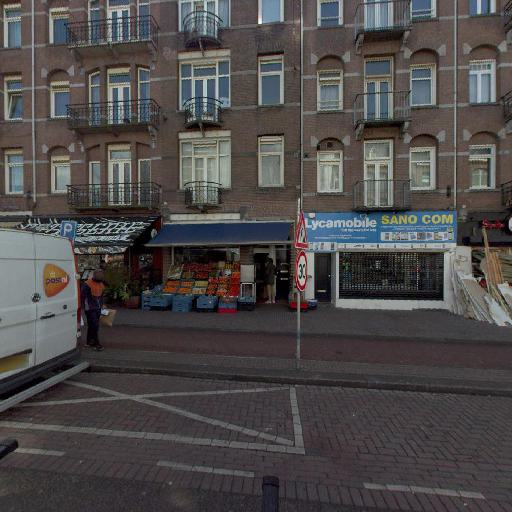
\includegraphics[width = 1.55in]{media/methodology/data_ex/extended/_left (2).jpg}} &
        \subfloat{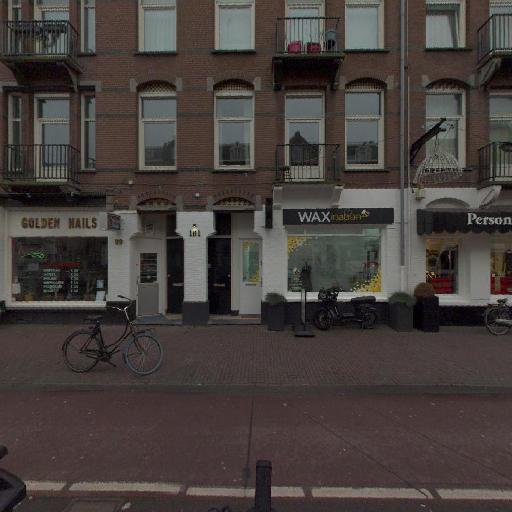
\includegraphics[width = 1.55in]{media/methodology/data_ex/extended/_left (4).jpg}} \\
        \subfloat{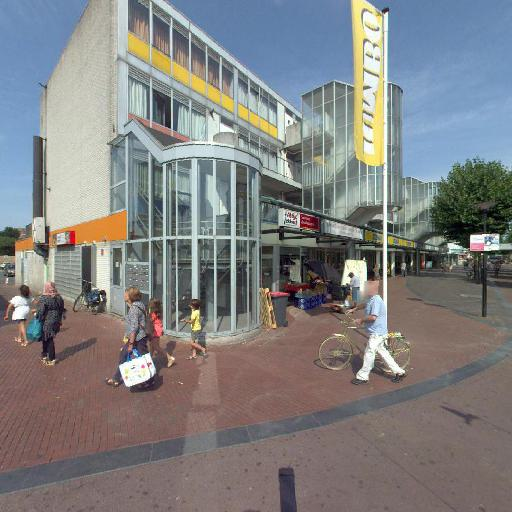
\includegraphics[width = 1.55in]{media/methodology/data_ex/extended/_right (1).jpg}} &
        \subfloat{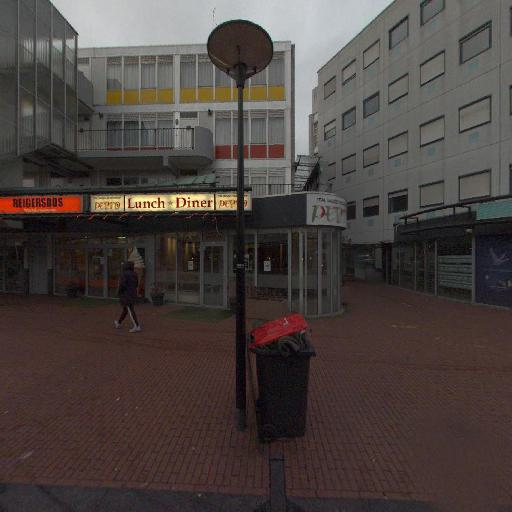
\includegraphics[width = 1.55in]{media/methodology/data_ex/extended/_right (2).jpg}} \\
    \end{tabular}
    \caption{Examples of left- and right-view images from the extended dataset.}
    \label{fig:panolr_example}
    \vspace{-5mm}
\end{figure}


\subsection{Experimental setup}

The data pipeline is visualized in Figure \ref{fig:pipeline}. This section outlines the implementations of CRAFT for scene text detection and the ResNets for classification.

\begin{figure*}
    \centering
    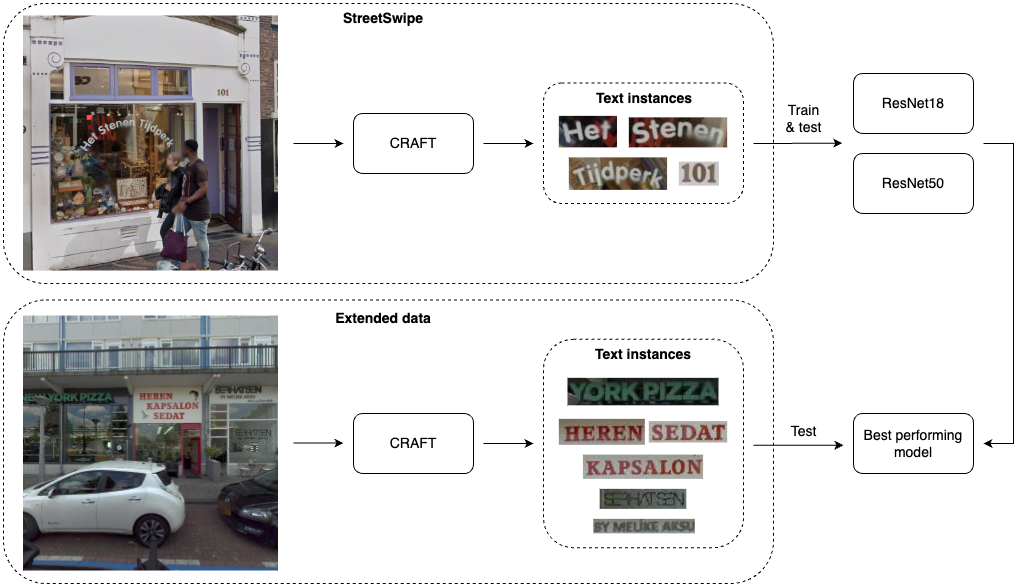
\includegraphics[width=0.9\textwidth]{media/methodology/Pipeline.png}
    \caption{Pipeline: Images of facades were first passed through the text detection model CRAFT to extract text instances. The ResNets were then trained and tested on instances from StreetSwipe. Subsequently, the best performing model was tested on instances from the extended data.}
    \label{fig:pipeline}
\end{figure*}


\subsubsection{CRAFT}

The first task was to detect and extract signage in the images of both datasets, using the pre-trained CRAFT model via the EasyOCR Python package \cite{noauthor_jaided_nodate}. More specifically, the \textit{detect} method was used, with text confidence threshold \textit{(text\_threshold)} set to 0.75, bounding box extension \textit{(add\_margin)} set to 0, and all other parameters set to their default values. Text instances were cropped out by their bounding boxes and grouped per class.

StreetSwipe returned 10079 instances in total, with 2610 gentrified instances (26\%) and 7469 non-gentrified instances (74\%). The instances varied in size, typically with width larger than height. The widths ranged from 8 to 1576, and heights ranged from 6 to 795 (see Appendix \ref{sec:apx:instances} - Figure \ref{fig:SS_ins_sz} for a visualization of the distributions). These text instances were used to train and optimize the classifier.

The extended dataset returned 2473 instances in total, with 1633 gentrified instances (66.03\%) and 840 non-gentrified instances (33.97\%). The instances varied in size, typically with width larger than height. The widths ranged from 8 to 510, and heights ranged from 4 to 191 (see Appendix \ref{sec:apx:instances} - Figure \ref{fig:pano_ins_sz} for a visualization of the distributions). These text instances were used to test the classifier for generalizability.


\subsubsection{ResNet}

StreetSwipe text instances were split into training, validation and test sets with 80:10:10 ratio. The data was randomly shuffled prior to splitting to maintain class distribution per split. Table \ref{tab:data_split} shows the size of each split as well as class distributions.

% {
% \setlength\intextsep{0pt}
\begin{table}[h!]
    \begin{tabular}{lrrrl}
    \toprule
            & \multicolumn{1}{r}{Total} &\multicolumn{1}{r}{Gentrified} & \multicolumn{1}{r}{Non-gentrified} \\ \cline{1-4}
Train       & 8063                      & 2092 (25.95\%)                & 5971 (74.05\%)      \\
Val         & 1008                      & 238 (23.61\%)                 & 770 (76.39\%)       \\
Test        & 1008                      & 280 (27.78\%)                 & 728 (72.22\%)       \\
    \bottomrule
    \end{tabular}
    \vspace{\baselineskip}
    \caption{Sample size per data split, per class}
    \label{tab:data_split}
    \vspace{-5mm}
\end{table}
% }

Images in the training set were randomly cropped and resized to 224x224, plus a random horizontal flip. Validation and test set images were resized and center-cropped to 224x224. All data was normalized with ImageNet's mean and standard deviation.

Model training was done in PyTorch. Both the ResNet18 and ResNet50 were initialized with pre-trained ImageNet1K-V1 weights. As a baseline, all the weights in the model were frozen and only the final layer was optimized, and no action was taken to account for class imbalance. Learning rate was set to 0.001, batch size was 32, and the model was trained for 50 epochs.

Next, the models were fine-tuned. PyTorch's WeightedRandomSampling was applied, with class weights calculated as 1/(class size). The loss function used was the cross entropy loss. The optimizer was stochastic gradient descent with a 0.9 momentum. StepLR learning rate decay scheduler was also implemented with a step size of 7 and gamma of 0.1. Hyperparameters tuning was done on the learning rate, batch size and number of training epochs.

\subsubsection{Visual inspection of model's outputs}
Random samples were taken from each of the following subsets of the output:

\begin{itemize}
    \item StreetSwipe's correctly classified signage per class with classification probability of 80\% and above. This showed the most distinguishing characteristics of gentrified and non-gentrified signage. In comparison to past research (Section \ref{subsec:related_signs}), conclusions were drawn on the extent to which the model could achieve similar results as qualitative analyses.
    \item StreetSwipe's misclassified signage, categorized by high ($ \geq 80\% $) and low (50-70\%) classification probability. Misclassifications showed characteristics of cases that the model failed to distinguish. This demonstrated the extent to which signage alone could fully determine (non-)gentrification to a computer vision model. It was expected that the varying degree of certainty would correspond to different visual patterns: misclassifications with high certainty would most likely have the same characteristics as the class they were assigned to, and misclassifications with low certainty would have less typical characteristics.
    \item Extended data's signage per class with classification probability of 80\% and above (irrespective of ground truth labels). It was expected that classifications follow the same characteristics in StreetSwipe, and by inspecting the corresponding facades we can get an idea of how well the model can detect perceptual gentrification via signage in unseen data.
\end{itemize}


\subsection{Evaluation}

\subsubsection{Scene text detection}

Since there was no bounding box annotations of the signage, evaluation was done by visual inspection.

\subsubsection{Classification}

Accuracy, precision, recall, and F1 score were calculated for the classifier. The macro-averaged metrics were used to compare models, and additionally metrics per class were calculated to examine the effect of class imbalance. The metrics were implemented using torchmetrics' MulticlassAccuracy, MulticlassPrecision, MulticlassRecall, and MulticlassF1Score. torchmetrics' ClasswiseWrapper was used to obtain metrics per class. 

% The formulas are as follow:

% \begin{align*}
%     Accuracy = \frac{TP+TN}{TP+TN+FP+FN} \\
%     Precision = \frac{TP}{TP+FP} & Recall = \frac{TP}{TP+FN} \\
%     F1 Score = \frac{2 * Precision * Recall}{Precision + Recall}
% \end{align*}

